\chapter{Background \& Related Work\label{chap:literature-review}}
This chapter is dedicated to background and work related to this project. The chapter covers advantages and disadvantages of several peer-to-peer mechanisms and current approach for communication between IoT devices in a smart city. Moreover, high-level description of blockchain mechanism with different approaches is provided.

\section{Smart City}
\quad Smart city is an urban area that produces and uses data from many sensors called Internet-of-Things (IoT) devices. These data collections help to improve life, health, comfort and resource management of the city. The difference between a regular city and a smart one is in IoT devices that collect all source of data and then these data collections are analyzed by artificial intelligence (AI) or pattern recognition algorithms. These results can late be used for above-mentioned improvements of cities. It is much more that one can imagine. One example that already has an impact in cities is a smart rubbish bin called Bigbelly\footnote{\url{http://bigbelly.com/}}. It senses the amount of rubbish inside and it sends a request for collecting the rubbish if it is getting full. Moreover, it can serve as public Wi-Fi hot-spot or broadcast useful information via Bluetooth.

IoT devices in cities are connected to a network mainly via Wi-Fi, Bluetooth, LoRa, 6LoWPAN, 4G or Ethernet technology. They usually do not have a lot of computing power. By its design, they try to be energy efficient because they are often battery powered. Therefore, these end-point devices are usually not suitable as peer-to-peer nodes. It is better if they can send data quickly and then sleep until the next time.

\section{Peer-To-Peer}
\quad Peer-To-Peer (P2P) system is different from a client-server system. Devices connected in a P2P system behave as both, server and client at once. Therefore, every peer in the P2P system can provide some of its resources. Be it bandwidth, storage capacities, files or CPU/GPU cycles. Nodes, connected devices to the P2P system, are considered unreliable and often even untrusted. The P2P system is generally a virtual overlay network on top of the physical topology of the network in which the node is connected. The application layer peers are able to communicate directly via the logical overlay network. Moreover, this communication network can be without central control. Based on the architecture of the overlay network we distinguish between three types of P2P systems. The first is centralised, the second is decentralised and the third is hybrid. Furthermore, based on the topology, a decentralised P2P system can be unstructured or structured \cite{vu_peer--peer_2010}. See Figure \ref{fig:P2P-architecture}.

\begin{figure}[ht]
	\centering
	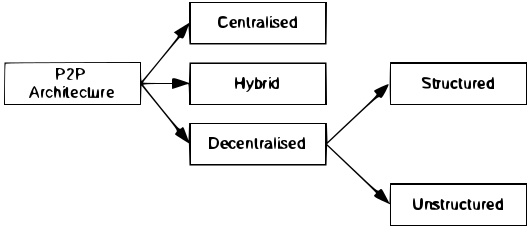
\includegraphics[width=0.7\textwidth]{images/p2p-architecture.png}
	\caption{\label{fig:P2P-architecture}P2P Architecture}
\end{figure}

\subsection{Centralised P2P system}
\quad Centralised P2P system combines both architecture patterns, client-server and P2P. A node first connects to the central server, often called a broker, in order to locate the desired resource on the P2P network or the server acts as a task scheduler that coordinates tasks among peers. The first example of such network is well known Napster \cite{noauthor_napster_2018}. It was originally founded as P2P music sharing service. A node connected to the Napster asked for a location of the desired resource and the server sends an address that has it. Unlike client-server architecture, once a node has the address it communicates directly with the peer that holds the required data. See Figure \ref{fig:centralised-p2p}. Napster was shut down and later reopened as a legal\footnote{\url{https://gb.napster.com/}} music streaming service. The second example is BOINC \cite{noauthor_boincpapers_nodate} or SETI@home \cite{noauthor_setihome_nodate}. In this case, the server acts as a task scheduler. Nodes fetch work units from the server directly. The advantages of this architecture good control over the network, cheap discovery of peers that have the required resource because the server holds the central index of all peers and their resources. On the other hand, the disadvantages are similar to client-server architecture. The server is a single point of failure. This type of P2P network does not scale well with a large number of nodes connected to the network. Finally, centralised P2P networks are not robust enough. A few examples of such P2P networks include Napster \cite{noauthor_napster_2018}, BOINC \cite{noauthor_boincpapers_nodate} and SETI@home \cite{noauthor_setihome_nodate}.

\begin{figure}[ht]
	\centering
	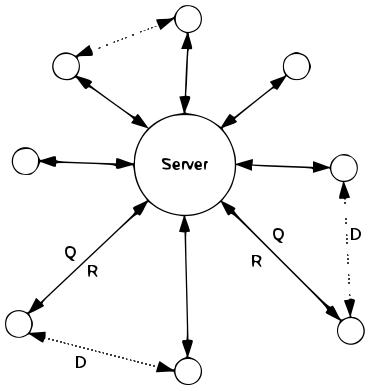
\includegraphics[width=0.3\textwidth]{images/centralised-p2p.png}
	\caption{\label{fig:centralised-p2p}(Q) node queries the server. (R) response from the server. (D) data exchange.}
\end{figure}

\subsection{Decentralised P2P system}
\quad Decentralised P2P system does not have any central index of resources and therefore no central point of failure. Every node in the decentralised P2P system has equal rights and responsibilities. A node has never complete knowledge about the network but only partial knowledge. If every node had complete information about all other peers in the network, every message would travel only one hop. On the other hand, every node would have to maintain a routing table of an O(N) size (where N is a number of nodes in a network). This would be unrealistic in P2P network of bigger size because each join and leave of a node would need to propagate to every peer in the network. The other extreme is if a node would have only two connections to each other in a ring topology. The cost of maintaining routing table would be minimal, but routing performance would be O(N). Decentralised P2P system radically improves robustness and scalability in comparison to a centralised P2P system. However, it introduces a new challenge of locating the desired resource (discovery service) on the P2P network. Two main approaches attempt to solve this issue. Based on the architecture of peers connecting in the overlay network, the approaches can be divided into structured and unstructured decentralised P2P systems. \cite{koegel_buford_p2p_2009}

\paragraph{Structured overlay network} maintains placement of resources or pointers to nodes that have desired resources under predefined rules. Generally, in structured P2P network this knowledge is maintained as distributed hash table (DHT\footnote{\url{https://en.wikipedia.org/wiki/Distributed_hash_table}}) \cite{korzun_structured_2013}. A DHT provides lookup service for connected peers in a similar way as a standard hash table. A node is responsible only for a subset of key-value pairs of the DHT in such a way that nodes joining and leaving cause a minimal amount of disruption.

As it was described previously, the number of connections that a node have with its peers (degree of a node) influences the routing performance and structure of the overlay network. Since networks can be modelled as graphs, they can be studied and evaluated with the help of graph theory \cite{loguinov_graph-theoretic_2003}. The table \ref{structured-graph-performance} and Table \ref{structured-graph-performance-2} show the specific properties of widely used structured P2P overlay networks. Therefore, It is important to choose the right one based on specific criteria.

\begin{table}[ht]
\centering
\caption{Asymptotic degree-diameter properties of the different graphs. (N is number of nodes in the graph)\cite{loguinov_graph-theoretic_2003}}
\label{structured-graph-performance}
\begin{tabular}{|l|l|l|}
\cline{1-3}
\textbf{Graph} & \textbf{Degree} & \textbf{Diameter D} \\ \cline{1-3}
de Bruijin & k & \(log_k N\) \\ \cline{1-3}
Trie & k+1 & \(2 log_k N\)  \\ \cline{1-3}
Chord & \(log_2 N\) & \(log_2 N\)  \\ \cline{1-3}
CAN & 2d & 1/2 dN 1/d \\ \cline{1-3}
Pastry & (b-1) \(log_b N\)  & \(log_b N\) \\ \cline{1-3}
Classic butterfly & k & 2 \(log_k N(1-o(1))\) \\ \cline{1-3}
\multicolumn{3}{|l|}{Note: Degree is a number of connection every node has.} \\ \hline
\multicolumn{3}{|l|}{Note: Diameter D is max distance (hops) that a message must travel.} \\ \hline
\end{tabular}
\end{table}

\begin{table}[ht]
\centering
\caption{Graph diameter for N = \(10^6\) (cells with a
dash indicates that the graph does not support the
corresponding node degree). \cite{loguinov_graph-theoretic_2003}}
\label{structured-graph-performance-2}
\begin{tabular}{|l|l|l|l|l|l|l|}
\hline
\textbf{k} & \textbf{de Bruijin} & \textbf{Trie} & \textbf{Chord} & \textbf{CAN} & \textbf{Pastry} & \textbf{Classic butterfly} \\ \hline
2 & 20 & - & - & huge & - & 31 \\ \hline
3 & 13 & 40 & - & - & - & 20 \\ \hline
4 & 10 & 26 & - & 1,000 & - & 16 \\ \hline
10 & 6 & 13 & - & 40 & - & 10 \\ \hline
20 & 5 & 10 & 20 & 20 & 20 & 8 \\ \hline
50 & 4 & 8 & - & - & 7 & 7 \\ \hline
100 & 3 & 6 & - & - & 5 & 5 \\ \hline
\end{tabular}
\end{table}

\quad The next thing that has to be considered while choosing the graph structure is churn rate\footnote{\url{https://en.wikipedia.org/wiki/Churn_rate}} on the P2P network. With every join and leave of a node, the routing table has to be updated. Usually, P2P networks such as Bittorrent\footnote{\url{http://www.bittorrent.com/}} have high churn rate. Majority of nodes do not stay connected for more than 1 hour \cite{stutzbach_understanding_2006}. This introduces higher maintenance cost than in P2P network where nodes have incentives to be connected for a longer time period. One example can be Skype in early days where the median lifetime of a node was 5.5 hours \cite{guha_experimental_2005}. As we can see churn rate is an important factor that needs to be considered while choosing the graph structure of P2P overlay network.

Another important thing affecting the performance of routing is locality. It is a relationship between overlay network and underlying physical network. If the physical network is not taken into account while constructing the overlay network, peers that are neighbours in the overlay network can be far away and a message has to do many hops in the physical network. Furthermore, peers that are on the same physical network can be very distant in the overlay network and a message has to do many hops in the overlay network. Consequently, this results in undesirable network traffic. \cite{zhang_construction_2004}. This problem is illustrated in Figure \ref{fig:localy-aware-overlay}.

\begin{figure}[ht]
	\centering
	\includegraphics[width=0.7\textwidth]{images/localy-aware-overlay-net.png}
	\caption{\label{fig:localy-aware-overlay}Illustration for locality-aware overlay and (b) randomly connected overlay \cite{zhang_construction_2004}}
\end{figure}

There are many implementations of DHT that were developed. CAN \cite{ratnasamy_scalable_2001}, Chord \cite{stoica_chord:_2003}, Pastry \cite{rowstron_pastry:_2001} and Tapestry \cite{zhao_tapestry:_2004} were the first one. Later, important improvements in terms of performance were made. CoralCDN\footnote{\url{http://www.coralcdn.org/}} achieved the improvement through "a latency-optimized hierarchical indexing infrastructure based on a novel abstraction called a distributed sloppy hash table, or DSHT" \cite{freedman_democratizing_2004}. DSHT helped also prevent hot-spot congestion (overloading a node when a specific key becomes very popular). Moreover, Coral maintained a hierarchy of DSHT clusters based on region and size and therefore, allowed "nodes to locate nearby cached copies of web objects without querying more distant nodes" \cite{freedman_democratizing_2004}. Also, important security improvements in DHT were made with the introduction of S/Kademlia \cite{baumgart_s/kademlia:_2007} that has high resilience against common attacks. It uses cryptographic puzzles in order to limit free NodeId generation. S/Kademlia also uses parallel lookups over multiple disjoint paths over the network. Initial evaluation has shown that even with 20\% of adversarial nodes in the network, there is still 99\% chance of a successful lookup \cite{baumgart_s/kademlia:_2007}. More comprehensive discussion about DHT and structured P2P is above the scope of this work. More information can be found in this book \cite{korzun_structured_2013}.



\paragraph{Unstructured overlay network} utilizes different approach how queries are forwarded between peers in the overlay network. Every node maintains only its own data and keeps track of its connected neighbours that it can send queries to. However, this maintenance of a list of neighbours comes with a huge cost of bandwidth. Approximately 55\% of all traffic is due to PING and PONG messages that serve for maintaining the list of neighbours \cite{ripeanu_mapping_2002}. As the name suggests there is no underlying structure that maps resources to nodes. Therefore, it is challenging to locate the desired resource because it is difficult to predict which node has it. Other difficulties are that there are no guarantees of completeness of answer (unless the whole network is searched) and response time \cite{vu_peer--peer_2010}. Examples of such P2P networks are famous Gnutella\footnote{\url{http://rfc-gnutella.sourceforge.net/}} and FastTrack\footnote{\url{https://en.wikipedia.org/wiki/FastTrack}}. There are two main algorithms used for unstructured P2P networks. They are flooding and random walk.

The first routing strategy used in unstructured overlay P2P network is flooding. Consider an overlay network in Figure \ref{fig:flooding-graph} where every node has degree between two and five (number of connected neighbours). With a higher degree, the distance between nodes reduces and a query has to do fewer hops in the overlay network. On the other hand, each node has to maintain a bigger list of its neighbours \cite{koegel_buford_p2p_2009}. This list of neighbours can be shared between nodes. Once a node requires specific information it queries all its neighbours because it does not know the location of requested information. This process repeats further at each queried node until requested information is found or the maximum number of hops is reached. This limit for the maximum number of hops a message can do is called time-to-live (TTL). The TTL is a parameter of every message (query) and at each hop, it is decremented by one. It prevents queries circulates endlessly. Each node also keeps a list of queries that answered and if it receives the same query again it simply drops it \cite{taylor_p2p_2009}.

\begin{figure}[ht]
	\centering
	\includegraphics[width=0.7\textwidth]{images/flooding-graph.png}
	\caption{\label{fig:flooding-graph}(A) Unstructured topology showing connections between peers and (B) query flooding to four hops. \cite{koegel_buford_p2p_2009}}
\end{figure}

The second approach used for routing queries in unstructured overlay P2P networks is random walk algorithm. It is very similar to flooding technique but it significantly decreases the communication cost. When a node issues or receives a query, it randomly selects neighbour (except the originator) and send the query further. However, the disadvantage is that the query processing time is very long. In order to improve the query processing time, the initiator could send \textit{k} messages instead of only one \cite{vu_peer--peer_2010}. See Figure \ref{fig:random-walk-graph}.

\begin{figure}[ht]
	\centering
	\includegraphics[width=0.7\textwidth]{images/random-walk-graph.png}
	\caption{\label{fig:random-walk-graph}(A) Random walk and (B) k-way parallel random walk, k=3. \cite{koegel_buford_p2p_2009}}
\end{figure}

\subsection{Hybrid P2P system}
\quad Hybrid P2P system combines both, centralised and decentralised P2P systems. The main advantage of the centralised P2P system is fast lookup time but it has scalability issues. On the other hand, decentralised P2P system scale better but it requires longer time in resource locating. In Hybrid systems a node can be selected as \textit{super node} also known as \textit{super peer} and serve other nodes as a server. There can be many criteria for selection of \textit{super node}. Be it bandwidth, number of connections, longevity and many others. Therefore, resource locating can be done in centralised fashion (through supernodes) and also decentralised fashion \cite{vu_peer--peer_2010}. It is clear that different P2P systems have their advantages and disadvantages. Therefore it is crucial to choose the right one or even combination of multiple approaches.

\begin{figure}[ht]
	\centering
	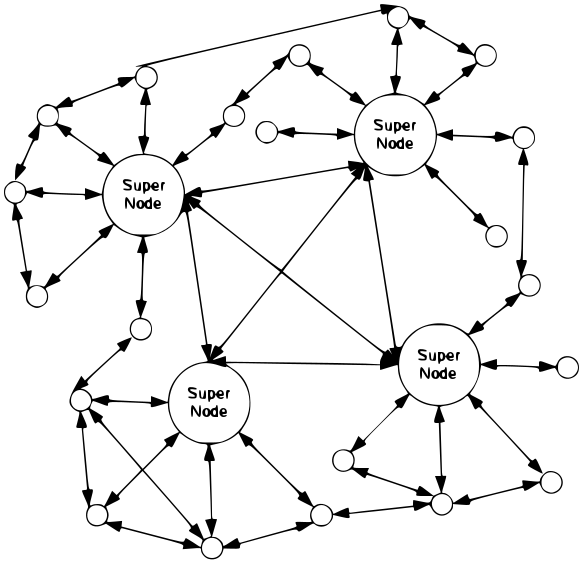
\includegraphics[width=0.5\textwidth]{images/hybrid-p2p.png}
	\caption{\label{fig:hybrid-p2p} Hybrid P2P overlay network. Super nodes act as server for peers.}
\end{figure}



\section{Distributed ledger}
\quad Distributed ledger technology (DLT) is a consensus of shared, synchronised and replicated records (financial or non-financial) spread across multiple geographic locations. There is no central data storage or single central authority. Users of DLT can use it to settle their transfers of data, money or assets without the need for trusted central authority. In traditional point of view, the central authority can be a financial institution such as a bank. DLT allows spreading the trust among participants instead of the traditional third party such as a bank. There are different types of DLTs. We can distinguish DLTs based on participation in the ledger, validation method and data structure of the shared records \cite{pinna_distributed_2016}.

\subsection{Permissioned VS Permissionless DLTs}
There are two types of participation in the ledger. The first is unrestricted also known as permissionless. The second is restricted also known as permissioned\cite{mattila_blockchain_2016}. In permissionless DLT anybody can participate in ledger update and validation. By definition, permissionless DLT is public. It means that the ledger is publicly available. On the other hand, in permissioned DLT only authorised participants can validate and update the ledger. Permissioned DLT can have private or public ledger \cite{pinna_distributed_2016}.

The choice of permissionless or permissioned DLT can have an effect on maintenance costs as well as the range of possibilities to enforce truthful behaviour of validators. In permissioned DLTs, validators are known and they can be punished for malicious behaviour. It can be outside of the DLT (e.g. legal contracts, fines, etc.) as well as inside the DLT (e.g. disqualification from validation process, credibility, etc.). However, in permissionless DLTs validators are unknown and may be punished only inside the DLT. Therefore, game theoretic tools are used in permissionless DLTs as well as public-key cryptography \cite{mattila_blockchain_2016}. Table \ref{properties-of-DLT} shows trade-offs between different types of DLT architectures. However, this table is only simplified version. While choosing the right DLT, it is crucial to get an excellent understanding of the specific DLT and its technical details.

\begin{table}[ht]
\centering
\caption{Trade-offs between different types of DLT architectures(simplified)}
\label{properties-of-DLT}
\begin{tabular}{|l|l|l|}
\cline{1-3}
\textbf{Properties of DLT} & \textbf{Permissioned} & \textbf{Permissionless} \\ \hline
Speed & Faster & Slower \\ \hline
Energy efficiency & Better & Worst \\ \hline
Scalability & Better & Worst \\ \hline
Censorship resistance & No & Yes \\ \hline
Tamper - proof & No & Yes \\ \hline
\end{tabular}
\end{table}

\subsection{Blockchain}
In 2008 Satoshi Nakamoto published a white paper called "Bitcoin: A Peer-to-Peer Electronic Cash System" \cite{nakamoto_bitcoin:_2008}. This paper revolutionized many industries. The idea of a cryptocurrency was not new but there was always a problem with double spend. Traditionally, this problem is solved via trusted third central authority such as bank instead of cryptographic proof. Satoshi Nakamoto did not invent new cryptographic methods, but he combines existing cryptographic methods, from 80's and 90's, in a new innovative way that allows the dawn of modern cryptocurrencies. This new invention is called a blockchain. Even though that in the original paper Satoshi Nakamoto did not mention the word blockchain, he describes the underlying principles of keeping transactions in \textit{blocks} that are \textit{chained} together via cryptographic hash (SHA256). He argued that the only way of preventing double spending is to know about all transactions. Even though that many people use terms blockchain and DLT interchangeably, it is considered to be only one type of DLT.

The fundamental principle of a generalised blockchain can be described as following. Records are grouped into blocks that one can imagine as a single page in a ledger. The next step is to create a cryptographic hash, such as SHA256, from this block and widely publishing it. The time when the hash is published is crucial. It proves that the records must have existed at the time to get into the hash. This is a timestamp of the block. Since each block contains a hash of the previous block, it forms a chain with each additional block reinforcing the ones before it. See Figure from the original Bitcoin paper \cite{nakamoto_bitcoin:_2008}.

\begin{figure}[ht]
	\centering
	\includegraphics[width=0.7\textwidth]{images/blockchain-satoshi.png}
	\caption{\label{fig:satoshi-blockchain}A chain of blocks with records \cite{nakamoto_bitcoin:_2008}.}
\end{figure}

In order to add a new block to the existing blockchain, the majority (in some cases at least 2/3) of the validators in the overlay P2P network have to agree on the newly created block. In permissioned blockchain, where we know the validators' identities and we can trust them, this proposal and validation of a new block is a straightforward process. On the other hand, in a permissionless blockchain where the validators are unknown and they can behave maliciously, we have to introduce countermeasures. An adversarial entity could create multiple nodes in the overlay P2P network and overvote the majority of honest nodes. This is known as Sybil attack\footnote{\url{https://en.wikipedia.org/wiki/Sybil_attack}}. In order to prevent this situation, Satoshi Nakamoto proposed a solution in a form of Proof-of-Work consensus algorithm. This is further discussed in Subsection \ref{consensus-algorithm-section}

A public blockchain is by its definition traceable and linkable. Everybody can see and track every record, source and destination address from the first (genesis) block up to the latest one. The first cryptocurrency that implemented and used public blockchain is Bitcoin\footnote{\url{https://bitcoin.org/}}. However, CriptoNote\footnote{\url{https://cryptonote.org/}} introduced the idea of completely anonymous transactions on a public blockchain. This is achieved with help of multiple cryptographic methods such as ring signature and ringCT, stealth address, ITP router and Pedersen commitment \cite{noether_ring_2015}. Explanation of how this type of anonymous blockchain works is out of the scope of this work. Examples of such anonymous cryptocurrencies are Monero\footnote{\url{https://getmonero.org/}}, AEON\footnote{\url{http://www.aeon.cash/}} and Bytecoin\footnote{\url{https://bytecoin.org/}}. In these cryptocurrencies, it is very difficult (almost impossible) to find the address of the sender and receiver, see any transaction or even see how much money was sent. Despite this, it is possible to validate the transaction and prevent double spending.

\subsection{Consensus Protocol}
\label{consensus-algorithm-section}
\quad Consensus algorithm is essential for DLT. Since the ledger is distributed, it is crucial to reach consensus between nodes about every single transaction. This is specifically difficult in unreliable environments such as P2P networks are. In fact, it turned out to be impossible to reach consensus even with one faulty process in an asynchronous environment where no assumptions about message delivery delays or relative speeds of processes are made \cite{fischer_impossibility_1985}. This proof is known as FLP impossibility. Therefore, all consensus protocols used in DLT are partially synchronous. Meaning that there are hard deadlines for validators.

In a case of permissioned DLT, any consensus protocol can be used to replicate the machine state. For example, a famous state machine replication protocol is Paxos\footnote{\url{https://en.wikipedia.org/wiki/Paxos_(computer_science)}}. This protocol is widely used in the industry for state machine replication. Its disadvantage is that it is difficult to understand and not Byzantine fault tolerant\footnote{\url{https://en.wikipedia.org/wiki/Byzantine_fault_tolerance}} (BFT) \cite{buchman_tendermint:_2016}. % use better source directly for Paxos
In 1999, Miguel Castro and Barbara Liskov published a paper "Practical Byzantine Fault Tolerance" (PBFT) that describes a new replication algorithm that is able to tolerate Byzantine faults \cite{castro_practical_1999}. This was a breakthrough because before there was not fast and efficient BFT protocol that could be used in real life. Recently a new effort has been made to improve the existing BFT state machine replication protocols. Tendermint\footnote{\url{https://tendermint.com/}} is one example that is already implemented as a pluggable consensus protocol for blockchains \cite{buchman_tendermint:_2016}. Another example of a blockchain that utilizes PBFT protocol is Hyperledger Fabric \cite{cachin_architecture_2016}. These examples consensus protocols solve only the issue of state machine replication. However, as it was mentioned previously, this would not be enough for permissionless DLTs due to the Sybil attack. In order to mitigate it, Satoshi Nakamoto proposed to use proof-of-work (PoW) for generating a new block on the blockchain \cite{nakamoto_bitcoin:_2008}.

Proof-of-work (PoW) is not a new idea. In 1992, Cynthia Dwork and Moni Naor invented the concept of "a computational technique for combatting junk mail in particular and controlling access to a shared resource in general" \cite{dwork_pricing_1992}.
In short, the requester of a service first has to do some computational work in order to use the requested service. Essentially, it introduces a cost of accessing the requested service via economic measure because the user's hardware, time and electricity are not for free. In the case of permissionless DLT, a Proof-of-Work is used to prevent the Sybil attack and flooding of the P2P network with fake new blocks. 

Bitcoin was the first cryptocurrency that used the idea of Proof-of-Work in the system. A node, in order to propose a new block, first have to solve a cryptographic puzzle. To be more specific, Bitcoin uses SHA256 cryptographic hash of a block (instead of a whole block it contains a Merkle tree root that is explained further). This hash of a newly proposed block must fulfil requirements of \textit{difficulty} which is a specific number of leading zero bits in the hash. This is achieved by adding a nonce that can be altered into the input of the hash. See Figure \ref{fig:satoshi-blockchain-pow} that shows how a previous hash, nonce and transactions creates a blockchain. With more zeros, the difficulty of a generating such a hash is exponentially increasing. The whole process is as follows. New transactions are broadcast to all nodes. Then each node collects new transactions into a block and it works on finding a difficult proof-of-work for its block. When a node finds it then it broadcasts the block with the hash to all nodes. Nodes should accept the block only if all the transactions are valid and they can easily verify that the work has been done by hashing the block and comparing those two hashes. Nodes express that they accept the new block by using the hash of the accepted block as a previous hash in a next block in the chain \cite{nakamoto_bitcoin:_2008}. This is a simplified description of consensus protocol with proof-of-work that Bitcoin uses.

Permissionless DLT works with an assumption that majority of validators are hones. In the case of Bitcoin and similar DLTs that utilize proof-of-work in their consensus protocol, not the majority of validators but the majority of the CPU power have to be honest. The longest chain represents the majority because there was invested the most of the proof-of-work effort. Therefore, the longest chain will grow the fastest and outpace any competing chains. If an attacker wants to modify a past block, she would have to redo the proof-of-work of the specific block and all blocks after it and overtake the chain produced by honest nodes. Satoshi Nakamoto showed that the probability of a slower attacker catching up decreases exponentially as subsequent blocks are added \cite{nakamoto_bitcoin:_2008}. Moreover, validators (miners) also have economic incentive, in form of reward, to continue the work and remain honest. Imagine that an attacker is in control of more computing power than all the honest nodes. She would have to decide between using the computation power to defraud people or earn new tokens (reward for creating new blocks and/or transaction fees). Remember that she would still have to spend a considerable amount of her own resources due to proof-of-work. By using it to steal back her payments, she would depreciate the market value of the tokens. Since this would be an undesirable situation for the attacker, she is disincentivised to do so.

\begin{figure}[ht]
	\centering
	\includegraphics[width=0.7\textwidth]{images/blockchain-pow-satoshi.png}
	\caption{\label{fig:satoshi-blockchain-pow}A chain of blocks with records that also contains a hash of the previous block and nonce \cite{nakamoto_bitcoin:_2008}.}
\end{figure}

Merkle tree is a cryptographic hash tree where every leaf node contains a hash of a data block and every node, that is not a leaf, contains a hash of its children's hashes \cite{merkle_protocols_1980}. Merkle tree is used to verify data that are transferred, stored or handled between computers or storages. It is often used in P2P networks (Gnutella\footnote{\url{http://rfc-gnutella.sourceforge.net/}}), file systems(Btrfs\footnote{\url{https://btrfs.wiki.kernel.org/}}, IPFS\cite{labs_ipfs_nodate}, ZFS\footnote{\url{https://en.wikipedia.org/wiki/ZFS}}) and DLTs (Bitcoin\cite{nakamoto_bitcoin:_2008}, Ethereum\footnote{\url{https://www.ethereum.org/}}, etc.). The advantage of using Merkle tree, instead of hashing the whole file, is that single block of data can be verified faster without the need of having all blocks of the file. To be more specific, in the case of a blockchain, separate transactions are hashed. These hashes are leaves of the graph as shown in the Figure \ref{fig:satoshi-merkle-tree}. Then it is not necessary to store all the transactions in a computer in order to verify a single transaction. This saves space and speed up verification process because the old blocks can be compacted by pruning the tree and leaving only the unspent transactions \cite{nakamoto_bitcoin:_2008}.

\begin{figure}[ht]
	\centering
	\includegraphics[width=0.7\textwidth]{images/merkle-tree-satoshi.png}
	\caption{\label{fig:satoshi-merkle-tree}Transactions are hashed in a Merkle Tree and root hash is included in the block hash instead of the whole block. For verifying if Tx3 is part of the block, we need only root hash, hash01, hash2 and the Tx3 \cite{nakamoto_bitcoin:_2008}.}
\end{figure}

Proof-of-stake (PoS) is another category of consensus algorithms that is used in permissionless DLTs. The basic concept is that validators have to make a secure deposit (bond some stake) if they want to participate in consensus. The weight of a vote depends on the size of validator's deposit (stake). In contrast to proof-of-work, proof-of-stake algorithms have significant advantages in terms of security, decreased the risk of centralization and energy efficiency. However, they have a major disadvantage that is "nothing at stake" problem discussed in the next paragraph. The first cryptocurrency that used proof-of-stake (with the combination of PoW) is Peercoin \cite{king_ppcoin:_2012}. Ethereum should also soon change its consensus algorithm to proof-of-stake. This new implementation is called Casper\footnote{\url{https://github.com/ethereum/casper}}.

This consensus algorithms have many advantages but in many implementations, including Peercoin, validators can be only rewarded for producing new blocks but not penalized. This is causing the problem of nothing at stake. In the situation where multiple chains are competing, the validator's incentive is to vote for every chain at the same time. Imagine a situation with two competing chains where the validator can vote on a chain A and get reward P = 0.9 or on a chain B where the reward is P = 0.1 or on both at once if possible. This is shown in Figure \ref{fig:nothing-at-stake}. This results in a violation of safety and there is no incentive to converge into a single growing blockchain \cite{noauthor_proof_nodate}.

\begin{figure}[ht]
	\centering
	\includegraphics[width=0.7\textwidth]{images/nothing-at-stake.png}
	\caption{\label{fig:nothing-at-stake} Nothing at stake problem. \cite{noauthor_proof_nodate}.}
\end{figure}

In comparison to proof-of-work, doing so would require splitting one's computing power in half. Therefore, this approach is not lucrative. It is shown in Figure \ref{fig:nothing-at-stake-pow}. In this situation when the validator votes for both competing chains, the reward for voting on chain A and B is decreased by 50\% and the combined reward is, therefore, smaller than voting only for original chain.

\begin{figure}[ht]
	\centering
	\includegraphics[width=0.7\textwidth]{images/nothing-at-stake-pow.png}
	\caption{\label{fig:nothing-at-stake-pow}Proof-of-work, splitting one's computing power in half  \cite{noauthor_proof_nodate}.}
\end{figure}

Nothing at stake can be prevented with a mechanism called \textit{slasher} that was first proposed by Vitalik Buterin (Co-Founder of Ethereum) \cite{buterin_slasher:_2014}. This mechanism penalizes validators that vote for multiple blocks simultaneously. When such situation happens then the validator's deposit is deduced appropriately. This mechanism is not simple to implement and it is still under heavy development for Ethereum Casper \cite{noauthor_proof_nodate}.

\begin{figure}[ht]
	\centering
	\includegraphics[width=0.7\textwidth]{images/nothing-at-stake-slasher.png}
	\caption{\label{fig:nothing-at-stake-slasher} Nothing at stake problem with slasher \cite{noauthor_proof_nodate}.}
\end{figure}

Some people argue that even without \textit{slasher} mechanism validators (stakeholders) have an incentive to act correctly and only vote for the original chain and not attacker's. The reason is that it is in their best interest to preserve the value of their investment because by supporting multiple chains at once the value of tokens on the market would decrease. On the other hand, this idea ignores that this incentive suffer from tragedy of commons\footnote{\url{https://en.wikipedia.org/wiki/Tragedy_of_the_commons}} problems \cite{noauthor_proof_nodate}.

Above mentioned consensus protocols are the most used one in DLTs. However, consensus protocols in DLTs are currently important research topic and we can expect new inventions and breakthrough. There are also proposed and being implemented many other categories of consensus protocols such as proof-of-space, delegated proof-of-stake, proof-of-activity, proof-of-importance, proof-of-burn and many combinations of them.

\subsection{Smart Contract}
\quad Smart contract was first proposed by Nick Szabo in 1995. The article "Smart Contracts: Building Blocks for Digital Markets" was published in magazine Extropy in 1996 \cite{szabo_smart_nodate}. He defined a contract to be "a set of promises agreed to in a meeting of the minds, is the traditional way to formalize a relationship." Contracts are mainly used in business relationships. Moreover, they are also used in personal relationships such as marriages, politics and other areas \cite{szabo_smart_nodate}. Szabo predicted in his article that digital revolution will dramatically change the traditional contracts. He called this new digital contracts "smart contracts". 

The basic principle of a smart contract is that contractual arrangements between parties are written in a programming language. By storing this piece of code that defines the contractual arrangements into a blockchain, the smart contract becomes temper proof, self-executing and automatically enforceable. This reduces the need for the trusted third party and human intervention in the case of disagreements. Therefore the whole process of around traditional contracts is made less risky and more cost-effective. In order to create a smart contract, it must be able to be represented in logical flow such as "If X Then Y Else Z" \cite{mattila_blockchain_2016}. Moreover, smart contracts must by deterministic otherwise nodes on the network would not reach consensus.

Ethereum was the first DLT that natively supported smart contracts. Ethereum provides a Turing complete virtual machine. It is called Ethereum Virtual Machine (EVM). Developers also created new programming language Solidity that is deterministic and suitable for smart contracts by its design \cite{noauthor_introduction_nodate}. Users can create their own contract, send them to Ethereum network where are replicated via BFT algorithm. For every execution of the contract a small fee, called Gas, has to be paid. Then the smart contract is sequentially executed on every node on the network.

Hyperledger Fabric is another example of a DLT that support smart contracts. In contrary to Ethereum, Fabric is permissioned blockchain. It rethinks the design and concepts used for permissionless DLTs and adapts them to suit better for permissioned DLT. It tackles existing limitations on permissionless DLTs such as execution throughput of smart contracts or the need for currency in public DLTs for smart contracts \cite{vukolic_rethinking_2017}.

\subsection{Distributed Ledger Technology in IoT \& Smart Cities}
\quad With the rise in popularity of modern cryptocurrencies many researchers and companies started to explore the unexplored possibilities of DLT. During my research of related work I encountered numerous research papers and articles that made false claims or misunderstood the problematics. Often "Blockchain" technology is used in many proposed solutions without any proper explanation or logical reasons. However, In this section I will focus on the work I consider to be very useful and inspiring for this project.

In \cite{christidis_blockchains_2016} authors did excellent summary of current blockchain technology and smart contracts. Moreover, they explored and discussed how smart contracts can be used in IoT and what should be considered for such deployment. One of the important things mentioned was that smart contracts are not legally binding (in permissionless DLT) and there is work being done towards solving this issue called "dual binding". On the other hand, I missed discussion about suitable consensus protocols for IoT devices. Despite it I consider it to be well written paper that served to me as introduction to this problematic.

In \cite{ozyilmaz_integrating_2017} an interesting concept was proposed to integrate Low-Power IoT devices to a Blockchain. Since IoT devices are often powdered by battery and they have low computation power, they are not suitable for blockchain integration. Authors proposed decoupled model where IoT devices communicate with a gateway that is connected to a blockchain network and acts as a node. This gateway (a full blockchain node) can be queried remotely via a smart contract running on the blockchain. As a proof of concept they used private Ethereum network and decreased PoW difficulty in order to reach faster speed. The code is available on GitHub \footnote{\url{https://github.com/kozyilmaz/blocky}}. It is good example how low power IoT devices can be integrated to a blockchain. However, in a real world scenario, a private Ethereum network would not be the best choice. Since the network is private, there is no need for PoW consensus and existence of currencies. Therefore, more efficient solutions, such as Hyperledger Fabric \cite{vukolic_rethinking_2017} could be used. A discussion about this is missing in the paper.

One of the closest related work to this project is \cite{ali_iot_2017}. In this paper authors proposed "a decentralized access model for IoT data, using a network architecture that we call a modular consortium architecture for IoT and blockchains."
With this architecture, they aim to provide IoT data privacy via blockchains and address the challenges associated with implementing blockchains to IoT. A single blockchain that would be  responsible for logging every IoT data operation would not scale well. Therefore, they broke down the network into smaller private network called \textit{sidechains}. These sidechains are interconnected via main \textit{consortium} network. A consortium network runs own blockchain. It is responsible for access control and  prevents any unauthorized access from one sidechain to another member of the consortium network. A sidechain is responsible for creation of legitimate IoT records and access control of incoming request transactions. These records are further stored in fully decentralised content addressed file system IPFS \cite{labs_ipfs_nodate}. A hash of this record is updated in the smart contract that is responsible for the data transaction. Moreover, the same decoupled pattern of IoT devices and blockchain is presented. In this scenario IoT devices hold encrypted communication with the gateway (called "validator node") that is running the smart contract. However, authors proposed this solution where "The private IoT network consists of IoT devices and one validator node running the sidechain". There is no benefit or reason of running the sidechain on a single computer. Either, there should be multiple nodes on the sidechain for decentralisation (increased reliability) or there is no need for the sidechain. Also there is no implementation of the proposed solution, but only network traffic and processing overhead of existing candidate blockchain solutions. The evaluated blockchains were Monax and Ethereum.

Similarly in \cite{shafagh_towards_2017}, authors proposed a solution where single blockchain is responsible for access control that is decoupled from storage layer. They consider IoT data to be streams and therefore introduced interesting concept of storing them in a specific data structure. Here are the data chunked, compressed and encrypted. Furthermore, these chunks are cryptographically chained together. This preserves the time-line of produced  data. They also advocate distributed data storage for saving these data streams. They relay on P2P overlay network and DHT that serves as general-purpose private key-value data store interface. This paper presents good solution to IoT secure data storage with promising initial evaluation results. However, I think that this proposed solution would not scale well due to single blockchain. Moreover, it does not integrate payments for shared (sold) IoT data.

There are also other papers that are related to this work and discusses IoT and blockchain integration in smart cities. 
CitySense: blockchain-oriented smart cities\cite{ibba_citysense:_2017}

Mind my value: a decentralized infrastructure for fair and trusted IoT data trading\cite{missier_mind_2017}

Towards an Optimized BlockChain for IoT\cite{dorri_towards_2017}


Slock.it\footnote{\url{https://slock.it/}}
Filament\footnote{\url{https://filament.com/}}
chain of things\footnote{\url{https://www.chainofthings.com/}}

